\documentclass{scrartcl}
\usepackage{dominatrix}
\begin{document}
  \begin{framed}
  \large
  CS 5220 Applications of Parallel Programming \hfill Fall 2015 \\
  Kenneth Lim (\href{mailto:kl545@cornell.edu}{kl545}) \hfill Computer Architecture Basics \hspace{-3ex}
  \end{framed}
  \begin{enumerate}
    \item See previous submission.
    \item See previous submission.
    \item In only serial execution, i.e. $p = 1$, the total time taken $T_s$ would be $t\tau$, where $\tau$ is the time taken per task. In pipelined execution with arbitrary $p$, the time taken for the very first task to complete is still $\tau$ because the pipeline is cold. However, each subsequent task will then come off the pipeline with a takt time of $\tau/p$. Thus the total time taken would be:
    \[
      T_p = \tau + \frac{(t-1)\tau}{p}
    \]
    The speedup is:
    \[
      \frac{T_s}{T_p} = \frac{t\tau}{\tau + \frac{(t-1)\tau}{p}} = \frac{pt}{p+t+1}
    \]
    \item The minimum serial time is 2.75h. The minimum parallel time is 2.25h.
    \item See \autoref{fig:local}.
      \begin{figure*}[ht!]
        \centering
        \begin{subfigure}[c]{.5\textwidth}
          \centering
          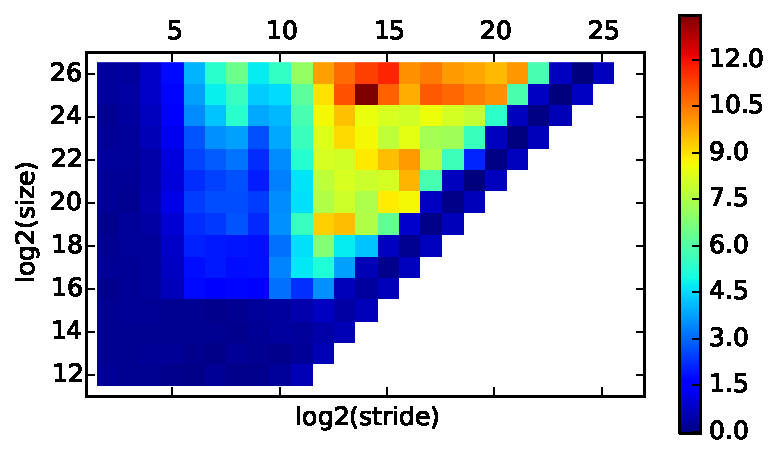
\includegraphics{local-timings-heat}
        \end{subfigure}%
        \begin{subfigure}[c]{.5\textwidth}
          \centering
          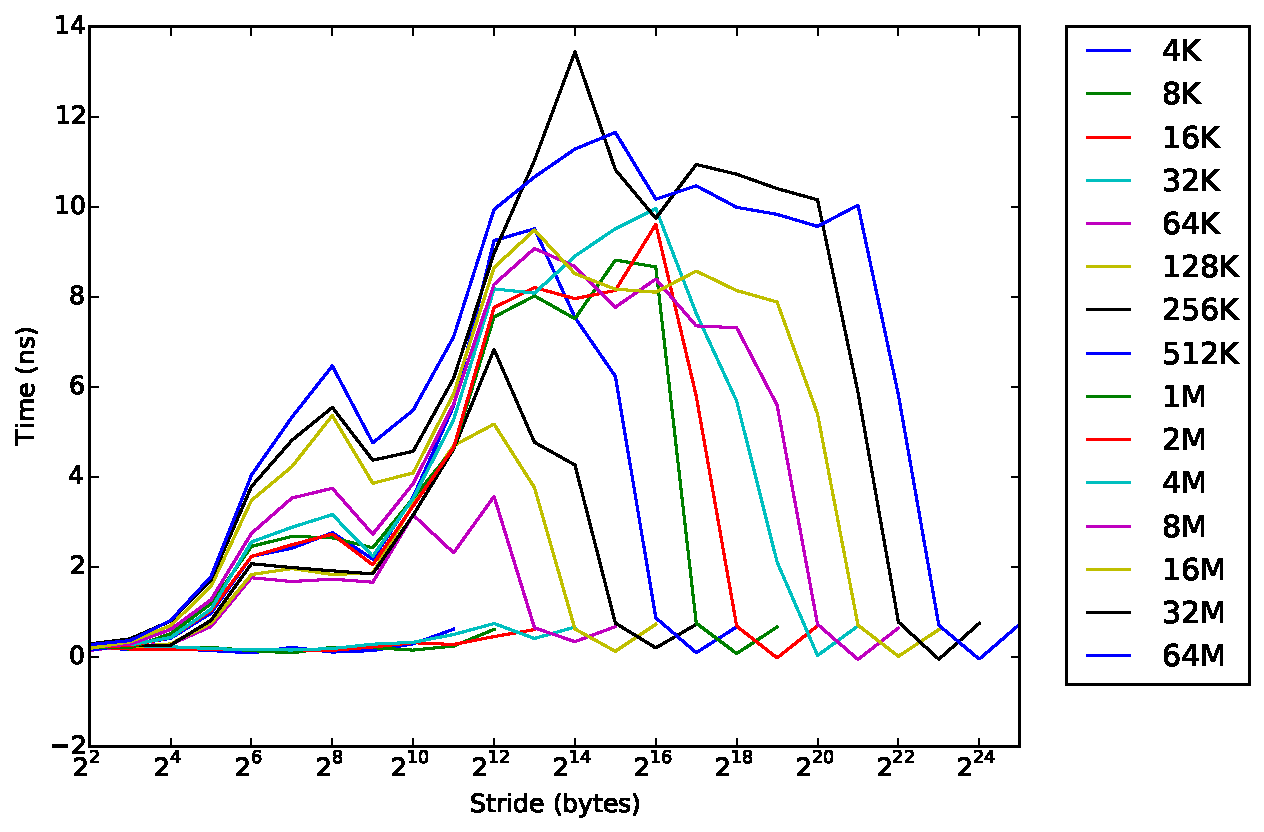
\includegraphics{local-timings-line}
        \end{subfigure}
        \caption{Membench results for the local system\label{fig:local}}
      \end{figure*}
    \item See \autoref{fig:cluster}.
      \begin{figure*}[ht!]
        \centering
        \begin{subfigure}[c]{.5\textwidth}
          \centering
          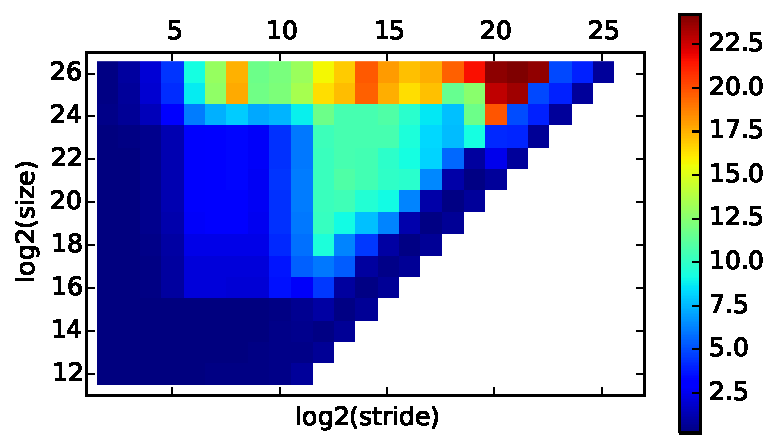
\includegraphics{totient-timings-heat}
        \end{subfigure}%
        \begin{subfigure}[c]{.5\textwidth}
          \centering
          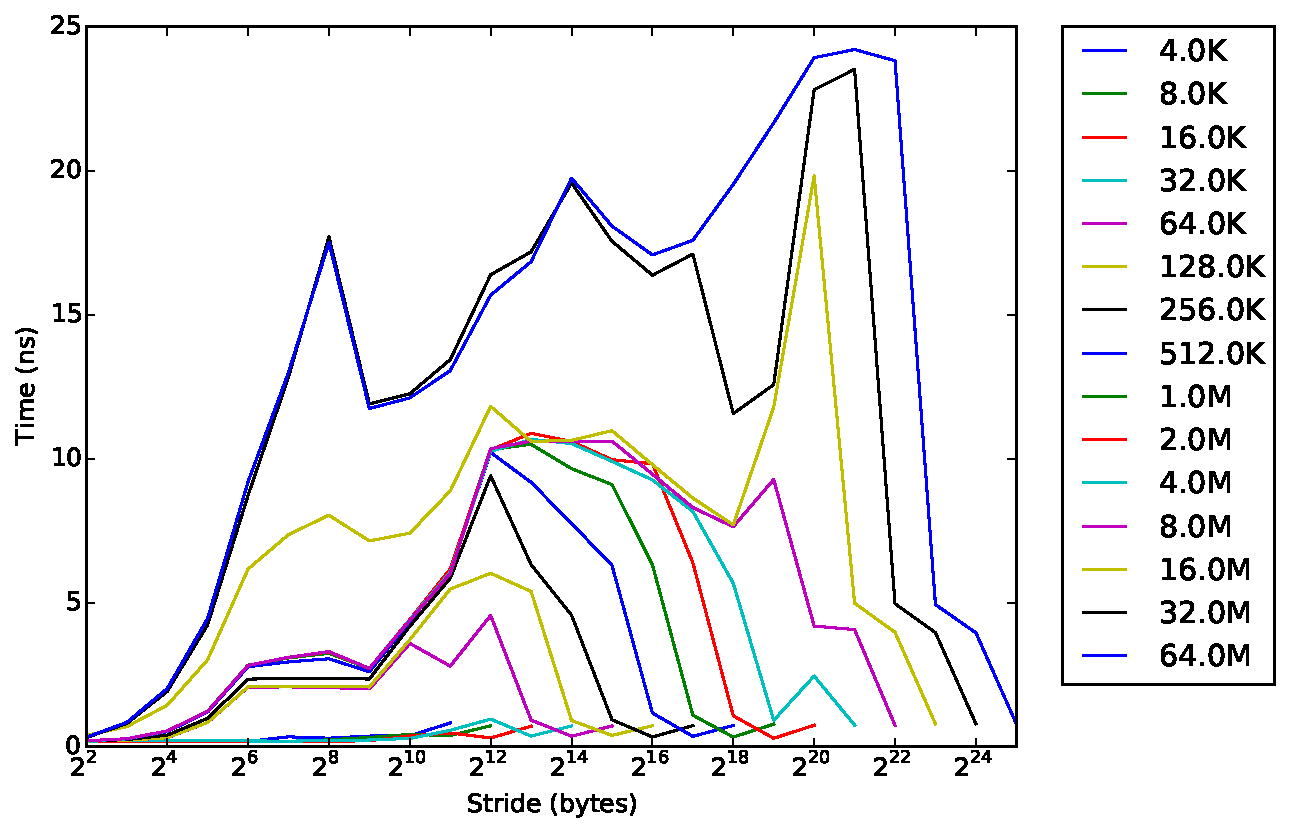
\includegraphics{totient-timings-line}
        \end{subfigure}
        \caption{Membench results for the totient cluster\label{fig:cluster}}
      \end{figure*}
    \item A caveat: when attempting to run \verb|centroid.c| verbatim from the course repo on the cluster, one found that it was consistently giving a timing of 0 for all three functions. The initial hypothesis was that the resolution of the default C timer was insufficient. Following up on Piazza, \verb|centroid.c| was modified to use the OpenMP timer, giving the following results:
    \begin{enumerate}[label=(\alph*)]
      \item 1.266918e-03
      \item 2.384777e-03
      \item 2.351441e-03
    \end{enumerate}
    Implementation B should be the slowest because it does not exploit memory locality or look-ahead, wheres Implementations A and C are faster because the compiler can optimize for array access from contiguous blocks of memory. Implementation A is understandably the fastest because it only has to go through the array once.
  \end{enumerate}
\end{document}
